In this section, we explore the potential of alternative decay schemes within the FedDecay framework.
Results in Section~\ref{sec: decay-method-decay} allow for more general sequences than exponential decay.
While exponential decay has been a focus, other strategies for scaling gradient emphasis during federated training could enhance performance by balancing initial model success, generalization, and rapid personalization.
We expand our analysis to include the use of linear decay for FedDecay.
We define linear decay as $\beta_j = \max \{1 - j (1 - \beta), 0 \}$, where $1 - \beta$ is employed for consistency aligning with FedSGD ($\beta = 0$) and FedAvg ($\beta = 1$).
Figure~\ref{fig: decay-schemes} illustrates the average test set accuracy for new and existing users across different decay schemes.
\begin{figure}
    \centering
    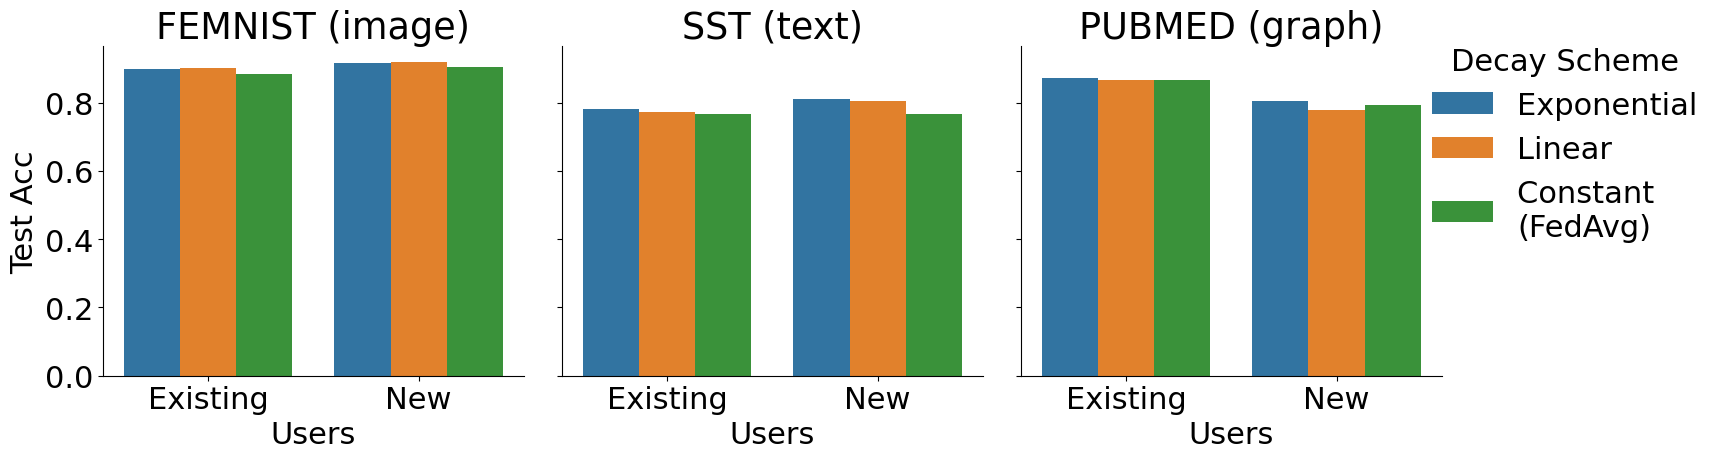
\includegraphics[width=\linewidth]{images/decay-scheme.png}
    \caption{
        Alternative Without-Round Decay Scheme Performance.
        Linear decay scheme can also provide improved performance over FedAvg.
        Within-round decay is generally an option for improving performance without additional computation or memory cost. 
    }
    \label{fig: decay-schemes}
\end{figure}

It is evident from the results that both exponential and linear decay schemes yield performance improvements over FedAvg.
While linear decay performs slightly worse than FedAvg on the new PUBMED user, it demonstrates robust performance on FEMNIST and SST2.
These findings underscore the potential for alternative decay schemes to enhance the overall model performance within the federated learning paradigm.
We emphasize that decay can be an effective tool for improving performance without additional cost.